\documentclass[conference]{IEEEtran}

\usepackage{booktabs}
\usepackage{graphicx}
\usepackage{url}
\usepackage{amsmath}
\usepackage{amssymb}

\title{Shape-Aware Sparse Traffic-Matrix Analytics for Reproducible GraphChallenge Anonymized Network Sensing}

\author{
\IEEEauthorblockN{Qifan Chen}
\IEEEauthorblockA{University of California, Santa Barbara\\
qifan\_chen@ucsb.edu}
}

\begin{document}
\maketitle

\begin{abstract}
The MIT/IEEE/Amazon GraphChallenge Anonymized Network Sensing track asks participants to construct and analyze anonymized source-to-destination traffic matrices from packet-derived data. We present a commodity-CPU reproducibility toolkit that lowers the entry barrier for student participants while making traffic-shape effects visible. The toolkit includes deterministic synthetic generators, exact sparse construction baselines, streaming/sketch heavy-hitter analytics, temporal bin summaries, and an early-stream method selector. On synthetic regimes up to 5,000,000 edge records, sparse direct construction wins on diffuse traffic while pandas pre-aggregation wins on highly duplicated hotspot traffic; a 50,000-record prefix correctly predicts the exact-method winner in all tested regimes. Streaming heavy-hitter recall is high only when candidate capacity is sufficient, exposing approximation failure modes, and controlled time-bin experiments identify volume, scanner, concentrated-destination, and distributed low-rate scan anomalies. The contribution is not full CAIDA-scale throughput, but a transparent, reproducible, student-oriented bridge between official GraphChallenge materials and commodity sparse-matrix experimentation.
\end{abstract}

\section{Introduction}
Network sensing tasks often begin with very large streams of packet or flow records. The Anonymized Network Sensing Graph Challenge frames these records as sparse source-to-destination traffic matrices suitable for graph and linear-algebra analysis~\cite{anonymizedNetworkSensing2024}. Official GraphChallenge submissions are paper-based and reward measured innovation in graph analysis software, hardware, algorithms, and systems~\cite{graphchallenge2026,graphchallengeSubmit2026}. This submission targets a complementary point in the GraphChallenge design space: not maximum throughput, but a reproducible, inspectable, low-dependency baseline that makes traffic-shape dependence and approximation risk measurable.

This work makes four contributions. First, it provides a commodity-CPU, low-dependency Python workflow from anonymized edge records to sparse traffic matrices and sensing summaries. Second, it adds a multi-regime synthetic benchmark that exposes when sparse direct construction, pandas pre-aggregation, and Python aggregation differ. Third, it includes a streaming/sketch path with explicit heavy-hitter recall diagnostics and candidate-capacity failure analysis. Fourth, it adds a time-bin and early-stream selector layer that turns traffic-shape measurements into interpretable anomaly and method recommendations.

\section{Related Work and Positioning}
GraphChallenge traffic-matrix tasks are closely aligned with sparse linear algebra. GraphBLAS defines graph analytics in terms of sparse matrix operations~\cite{buluc2017graphblas}, and SuiteSparse:GraphBLAS shows how such ideas can be implemented efficiently~\cite{davis2019suitesparse}. Recent reference-implementation work for GraphChallenge emphasizes improving official pipeline clarity, adaptability, and performance~\cite{voloshchuk2026improving}. Our work is complementary: it does not replace a high-performance reference implementation, but focuses on a student-facing CPU toolkit with synthetic regime controls, streaming failure diagnostics, temporal anomaly summaries, and online method selection.

Network measurement has also long used sketches and heavy-hitter algorithms for high-rate streams, including Count-Min Sketch~\cite{cormode2005countmin}, Misra-Gries summaries~\cite{misra1982finding}, SpaceSaving/top-$k$ stream tracking~\cite{metwally2005spacesaving}, and sketching systems for network measurements~\cite{kumar2004sketching}. Traffic anomaly studies show that feature distributions and traffic shape can be as important as aggregate volume~\cite{lakhina2005mining}. This package connects those ideas to the GraphChallenge setting while keeping the claim boundary conservative.

\subsection{Student Innovation}
The student innovation is not a new hardware record or a claim of full CAIDA-scale throughput. It is a low-barrier reproducibility package for commodity CPUs: deterministic data generation, exact command-line workflows, transparent pandas and Python baselines, multi-regime sparse traffic-matrix benchmarks, streaming/sketch analytics, time-bin anomaly summaries, and interpretable outputs that expose heavy hitters, source and destination structure, traffic concentration, and temporal bursts. The implementation is intentionally not optimized with GPU, C++, or distributed GraphBLAS, making it a baseline rather than a performance ceiling.

\section{Approach}
The input format is an anonymized edge table with source identifier, destination identifier, and a numeric traffic weight such as bytes or packets. The pipeline factorizes source and destination labels, constructs a SciPy coordinate matrix, converts it to compressed sparse row format, and sums duplicate source-destination pairs. This yields a sparse matrix $A \in \mathbb{R}^{m \times n}$ where $A_{ij}$ is the aggregate traffic from source $i$ to destination $j$.

The implementation then computes analytics intended to be useful for network sensing:
\begin{itemize}
\item matrix size, nonzeros, density, and total traffic;
\item top-$k$ heavy hitter source-destination pairs;
\item source and destination degree and strength distributions;
\item entropy of source strength, destination strength, and edge weights;
\item a largest singular value as a lightweight spectral summary;
\item a Gini coefficient of nonzero edge weights as a concentration statistic.
\end{itemize}

The repository includes three exact construction methods. The primary method builds a sparse matrix directly from edge records. A pandas baseline first groups by source and destination. A pure Python dictionary baseline aggregates pairs with a counter-like loop for small inputs. All exact methods are checked for output equivalence on the same synthetic inputs.

The new streaming path processes edge records sequentially. It keeps exact source and destination strength summaries, a fixed-size Count-Min Sketch for approximate edge weights~\cite{cormode2005countmin}, and a bounded candidate tracker inspired by streaming heavy-hitter algorithms~\cite{misra1982finding}. The streaming path is intentionally evaluated as an online approximation rather than a faster replacement for optimized SciPy sparse construction. Its main diagnostic is top-$k$ heavy-hitter recall against the exact sparse matrix.

The time-bin path groups the same edge records by a supplied \texttt{time\_bin} field and computes total traffic, nonzeros, source and destination entropy, edge-weight Gini, top-edge share, top-source share, top-destination share, and source/destination coverage. A robust positive-deviation score summarizes bins with unusually high traffic volume, fanout, concentration, or coverage. Network sensing is not only whole-matrix aggregation; temporal aggregation can expose burst, scan, or sudden concentration patterns that disappear in a single summed matrix.

Finally, the online selector uses only an early stream prefix to compute duplication rate, estimated nonzero growth, source and destination entropy, edge Gini, top-edge share, and top source/destination concentration. It applies the rule table below and is meant to make traffic-shape dependence visible, not to replace profiling.

\noindent\textbf{Algorithm 1: early-stream selector.}
Given a prefix, compute duplication rate $d$, nnz growth $g$, edge Gini $G$, top-edge share $e$, and top source/destination share $s$. If $d \geq 0.55$ or $G \geq 0.82$ or $e \geq 0.01$ or $s \geq 0.05$, recommend pandas pre-aggregation and mark sketch heavy hitters as plausible for concentrated traffic. Else if $d \leq 0.20$ and $g \geq 0.80$, recommend sparse direct construction and mark fixed-candidate sketches unsafe for top-$k$ discovery. Otherwise, recommend sparse direct construction and profiling before using sketches. These thresholds are empirical and chosen only to separate the synthetic regimes used in this submission; they are not claimed to be universal.

\section{Reproducibility Package}
The package is intentionally small. The main scripts are:
\begin{itemize}
\item setup, sample-generation, and sparse-analysis scripts;
\item benchmark and figure scripts for exact, streaming, sensitivity, and selector experiments;
\item a time-bin anomaly script for controlled network-sensing scenarios;
\item an optional reference wrapper and a local GraphChallenge-paper-style formula comparison.
\end{itemize}

The synthetic generator is not a substitute for CAIDA-scale data. It provides four regimes: \texttt{hotspot\_zipf}, \texttt{community\_bursty}, \texttt{scanner\_fanout}, and \texttt{uniform\_sparse}. It also exposes controlled knobs for edge count, source and destination counts, target nonzeros or density, duplication rate, Zipf skew, community structure, scanner fanout, and temporal bursts. These controls make the local benchmark runnable without protected downloads or multi-gigabyte packet captures while still testing multiple sparse traffic shapes.

\section{Experiments}
Experiments were run on a MacBook Air with Apple M3 CPU, 8 cores, 16 GB RAM, macOS 26.5.1 arm64, Python 3.9.6, NumPy 2.0.2 with Apple Accelerate BLAS/LAPACK, SciPy 1.13.1, pandas 2.3.3, and matplotlib 3.9.4. No GPU, distributed runtime, or manual BLAS thread pinning is used. The small benchmark uses generated edge tables at 5,000, 25,000, and 100,000 records, with three repeats and three exact methods. The large benchmark uses 1,000,000 and 5,000,000 records, one repeat, and two scalable exact methods. Reported construction and analytics runtimes exclude synthetic data generation and disk I/O unless otherwise stated; the input edge table is already resident in memory. The benchmark also records edges per second, nonzeros per input edge, and process peak RSS divided by input edges. The streaming benchmark uses 25,000, 100,000, and 500,000 records. Sensitivity studies vary sketch width and candidate capacity at 100,000 records. The method-selector experiment uses the first 50,000 records of each generated 5,000,000-edge stream and compares its recommendation with the saved fastest exact method. Time-bin experiments inject volume burst, scanner fanout, concentrated-destination, and distributed low-rate scan events into synthetic bins. A small official-format smoke test writes and reloads a GraphBLAS-style Matrix Market sparse coordinate matrix and checks shape, nonzeros, and total weight against the edge-table pipeline. Commands are exposed through the repository Makefile.

The key correctness check is output equivalence. For every benchmark row, the matrix produced by the method under test is compared with the sparse direct matrix. Total traffic is also compared. A benchmark row is marked valid only when both checks pass.

\section{Results}
Figure~\ref{fig:runtime} shows small benchmark mean runtime by input size, regime, and method. Figure~\ref{fig:large} shows the large benchmark. The exact numbers should be regenerated on the submission machine before final paper upload because Python package versions and CPU hardware affect the results.

\begin{figure}[t]
\centering

\includegraphics[width=\linewidth]{../figures/benchmark_runtime.png}
\caption{Mean runtime for sparse traffic-matrix construction and summary analytics on reproducible synthetic inputs. The plot is a smoke-scale comparison; large-regime throughput is summarized separately in Table~\ref{tab:large}.}
\label{fig:runtime}
\end{figure}

\begin{figure}[t]
\centering
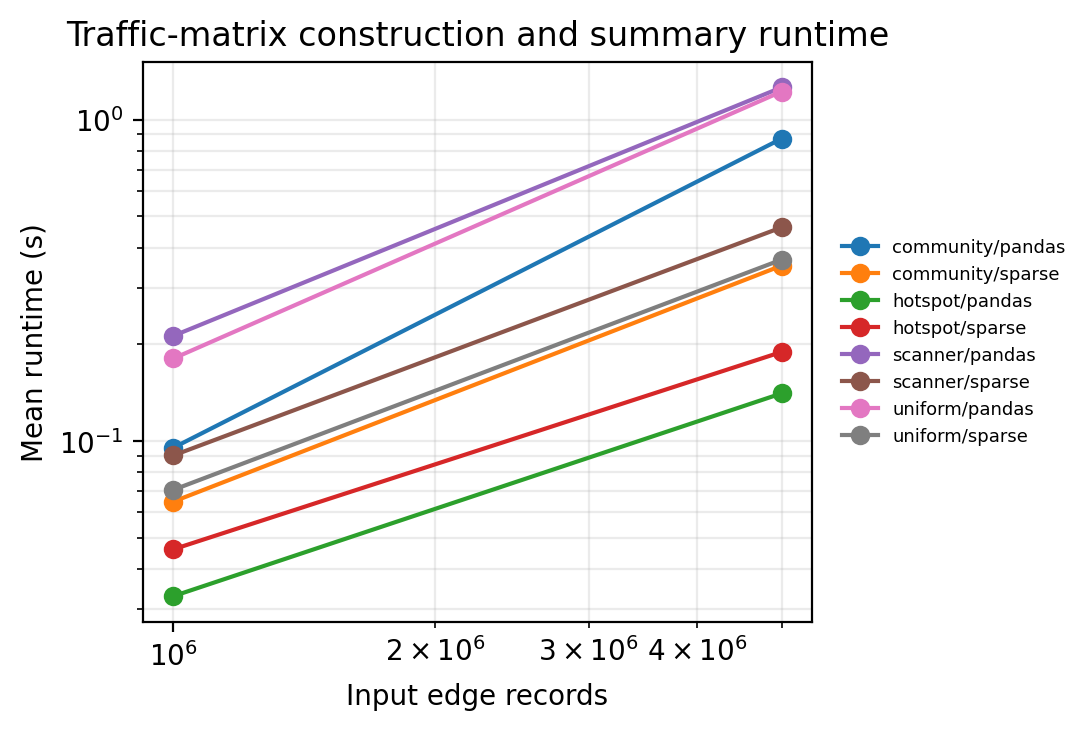
\includegraphics[width=\linewidth]{../figures/benchmark_large_runtime.png}
\caption{Large commodity-CPU benchmark up to 5,000,000 edge records across four synthetic regimes. The winner changes with duplication and nnz growth, so a single construction strategy is not uniformly best.}
\label{fig:large}
\end{figure}

\begin{figure}[t]
\centering
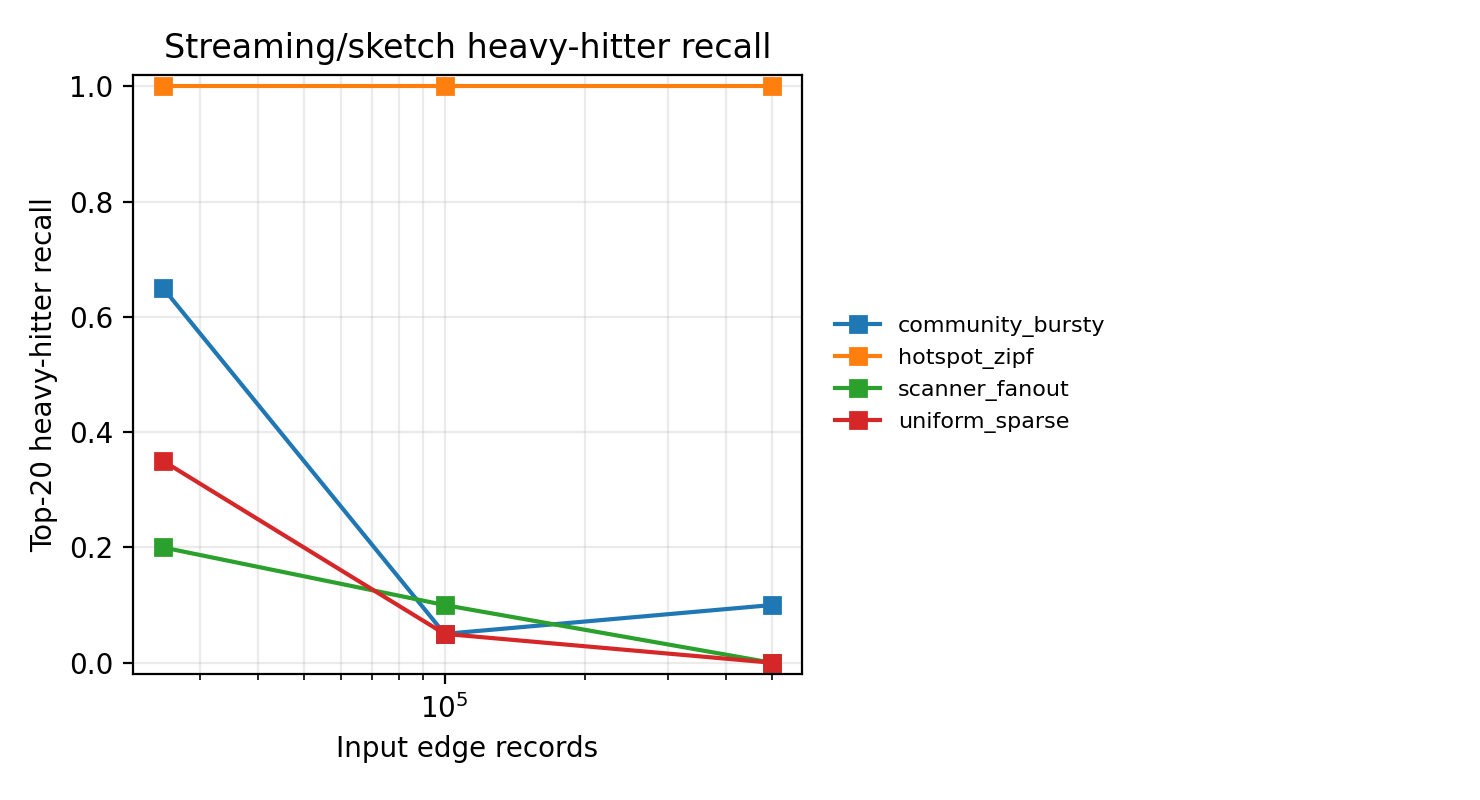
\includegraphics[width=\linewidth]{../figures/streaming_topk_recall.png}
\caption{Streaming/sketch top-20 heavy-hitter recall. The same fixed-size sketch is reliable for concentrated hotspot traffic but fails to discover diffuse heavy hitters, showing that sketch width alone is insufficient without adequate candidate tracking.}
\label{fig:streaming}
\end{figure}

\begin{figure}[t]
\centering
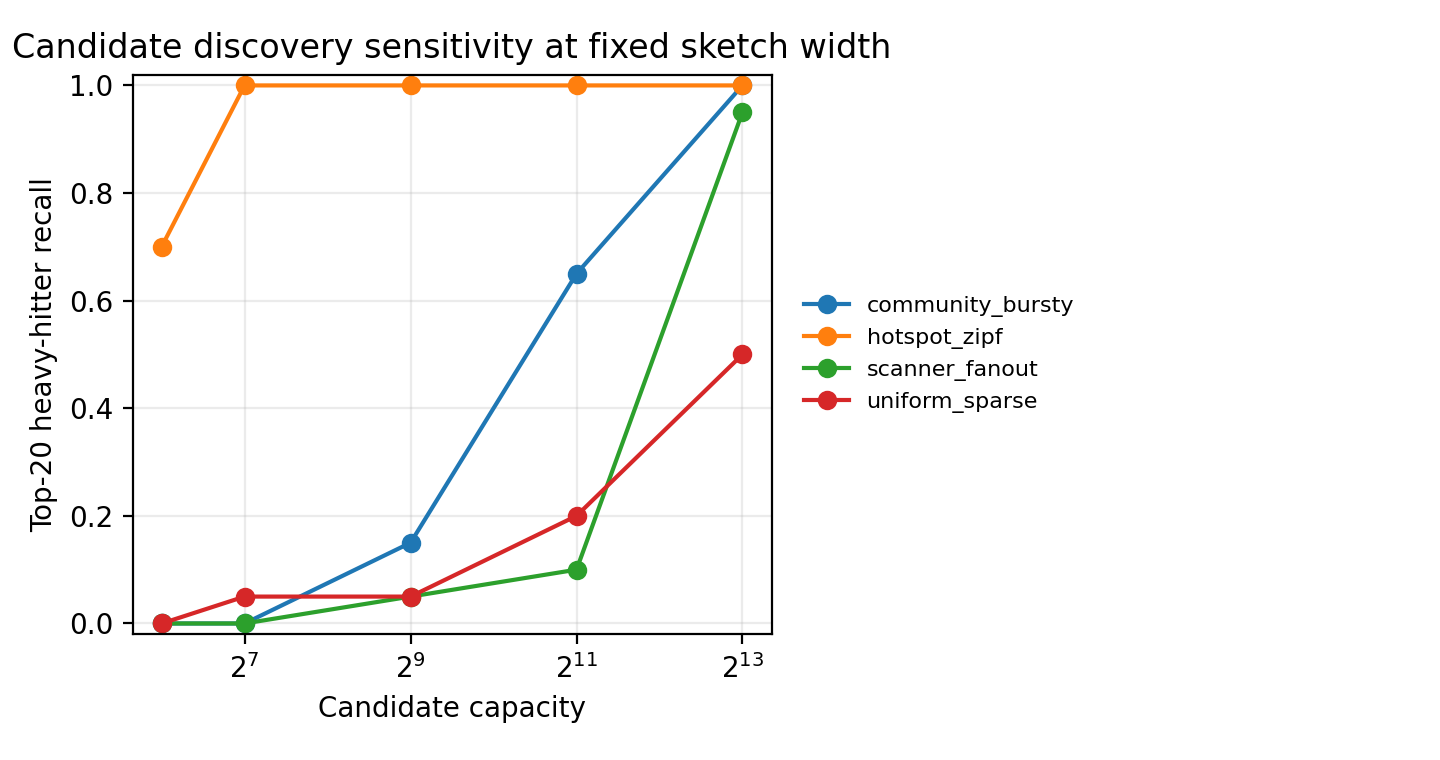
\includegraphics[width=\linewidth]{../figures/candidate_sensitivity.png}
\caption{Candidate-capacity sensitivity at fixed sketch width. Candidate capacity, rather than sketch width, is the limiting factor for diffuse heavy-hitter discovery.}
\label{fig:candidate}
\end{figure}

\begin{figure}[t]
\centering
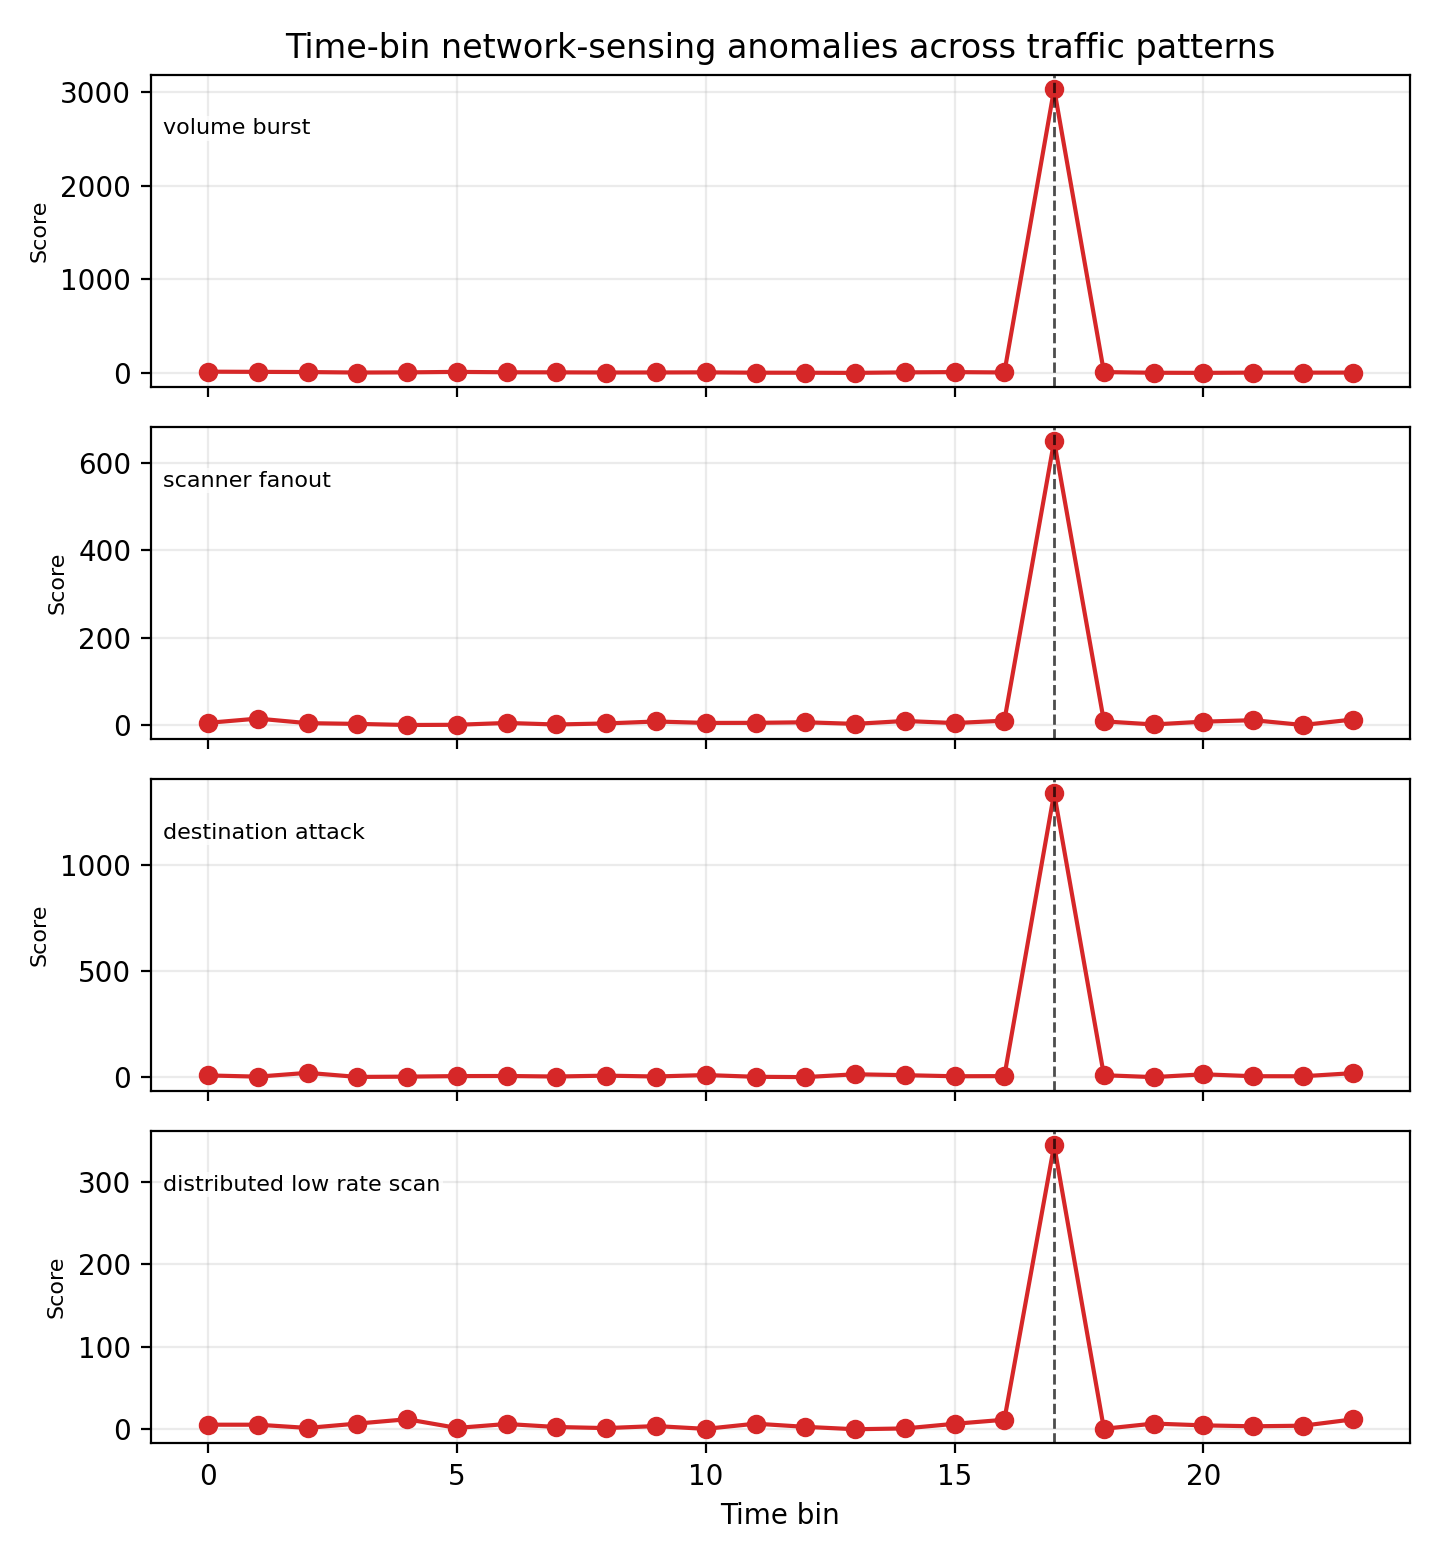
\includegraphics[width=\linewidth]{../figures/timebin_anomaly.png}
\caption{Time-bin sensing curves for four controlled network patterns. The dashed line marks the injected anomaly bin; different features expose volume burst, scanner fanout, destination concentration, and distributed low-rate scan behavior.}
\label{fig:timebin}
\end{figure}

Table~\ref{tab:large} reports the 5,000,000-edge large benchmark. The regimes differ substantially: hotspot traffic has 222,097 nonzeros and high concentration, while uniform sparse traffic has 4,997,173 nonzeros and density 0.0011. Sparse direct construction is faster than pandas groupby in community, scanner, and uniform regimes. In the hotspot regime, pandas groupby is faster on this machine, which is a useful negative result: the best construction path depends on traffic shape and duplication rate. The table reports total measured construction plus analytics time and throughput for in-memory edge tables.

\begin{table}[t]
\centering
\caption{Large benchmark at 5,000,000 input edges. Runtime excludes synthetic generation and disk I/O.}
\label{tab:large}
\begin{tabular}{lrrrrr}
\toprule
Regime & nnz/edge & Sparse & Sp. M/s & pandas & pd. M/s \\
\midrule
Hotspot & 0.044 & 0.189 & 26.4 & 0.141 & 35.5 \\
Community & 0.451 & 0.351 & 14.2 & 0.873 & 5.7 \\
Scanner & 0.992 & 0.462 & 10.8 & 1.261 & 4.0 \\
Uniform & 0.999 & 0.367 & 13.6 & 1.224 & 4.1 \\
\bottomrule
\end{tabular}
\end{table}

Table~\ref{tab:streaming} summarizes the streaming/sketch result at 500,000 edges. The Count-Min Sketch uses 327,680 bytes. It recovers all top-20 heavy hitters in hotspot traffic with median relative error below 0.001, but recall falls to 0.10 for community traffic and 0 for scanner and uniform regimes. A width sweep showed that increasing sketch width from 512 to 32,768 reduces hotspot median weight error from 0.0405 to 0 but does not improve diffuse-regime recall at fixed candidate capacity. Figure~\ref{fig:candidate} shows the missing factor: increasing candidate capacity from 64 to 8192 raises community recall from 0 to 1.00 and scanner recall from 0 to 0.95, but the 8192-candidate diffuse runs take about 23.2--25.0 seconds at 100,000 edges. In this Python implementation, streaming is slower than SciPy sparse construction, so its value is bounded-memory online processing and a clear approximation baseline, not raw speed.

\begin{table}[t]
\centering
\caption{Streaming/sketch heavy-hitter result at 500,000 edges.}
\label{tab:streaming}
\begin{tabular}{lrrr}
\toprule
Regime & Stream Time & Recall & Median Err. \\
\midrule
Hotspot & 5.31 & 1.00 & 0.0003 \\
Community & 9.81 & 0.10 & 1.0000 \\
Scanner & 10.23 & 0.00 & 1.0000 \\
Uniform & 10.17 & 0.00 & 1.0000 \\
\bottomrule
\end{tabular}
\end{table}

Table~\ref{tab:selector} reports the online method-selector experiment. From only the first 50,000 records, the selector identifies the hotspot regime as high-duplication and concentrated, recommends pandas pre-aggregation, and matches the saved 5,000,000-edge winner. For community, scanner, and uniform regimes, nonzeros grow almost one-for-one with the stream and the selector recommends sparse direct construction, again matching the saved winner. This result is useful because it turns the benchmark into an online decision rule with visible failure boundaries: sketches are plausible for concentrated heavy hitters, but diffuse traffic should default to exact sparse construction or use much larger candidate sets.

\begin{table}[t]
\centering
\caption{Early-stream method selector at 50,000 observed records, compared with 5,000,000-edge exact-method winners.}
\label{tab:selector}
\begin{tabular}{lrrll}
\toprule
Regime & Dup. & Top edge & Rec. & Winner \\
\midrule
Hotspot & 0.775 & 0.0948 & pandas & pandas \\
Community & 0.010 & 0.0007 & sparse & sparse \\
Scanner & 0.000 & 0.0003 & sparse & sparse \\
Uniform & 0.000 & 0.0003 & sparse & sparse \\
\bottomrule
\end{tabular}
\end{table}

Table~\ref{tab:reference} reports compatibility validation rather than a speed contest. The Matrix Market smoke test reloads a GraphBLAS-style sparse coordinate matrix and exactly matches the edge-table sparse matrix on shape, nonzeros, and total weight. The formula check compares our pipeline with a local implementation of GraphChallenge-paper-style sparse sensing formulas on a 100,000-edge community sample. This is not the full official GraphChallenge reference repository, but it verifies that core scalar quantities agree before performance claims are interpreted.

Figure~\ref{fig:timebin} shows the time-bin anomaly experiment. In all four scenarios, the injected bin is the top-ranked bin by the robust anomaly score. The volume-burst case raises total traffic to 1.11B bytes versus a typical-bin median of 22.7M. The scanner-fanout case has top-source share 0.0469; the concentrated-destination case has top-destination share 0.1076; and the distributed low-rate scan has 16,806 nonzeros versus a typical median of 4,869. This is still synthetic, but it is closer to network sensing than a single toy spike because different features explain different event types.

\begin{table}[t]
\centering
\caption{Compatibility validation for official-format and reference-formula paths.}
\label{tab:reference}
\begin{tabular}{llrrr}
\toprule
Check & Input & nnz & Weight & Status \\
\midrule
Matrix reload & 10k MM & 4,747 & 66.1M & match \\
Formula scalars & 100k edge & 75,952 & 648.3M & match \\
\bottomrule
\end{tabular}
\end{table}

Table~\ref{tab:methodsummary} summarizes the selector output in reviewer-facing terms. It separates exact-method choice from sketch safety: pandas is recommended only when early traffic is highly duplicated and concentrated, while fixed-candidate sketching is marked unsafe for diffuse regimes even when exact sparse construction remains fast.

\begin{table}[t]
\centering
\caption{Method recommendation summary from the early-stream selector.}
\label{tab:methodsummary}
\begin{tabular}{llll}
\toprule
Regime & Method & Sketch safety & Reason \\
\midrule
Hotspot & pandas & safe & concentrated \\
Community & sparse & unsafe & diffuse candidates \\
Scanner & sparse & unsafe & fanout/diffuse \\
Uniform & sparse & unsafe & nnz grows with stream \\
\bottomrule
\end{tabular}
\end{table}

The current benchmark supports three conservative observations. First, all local exact construction paths produce equivalent aggregate matrices on the tested inputs, which is necessary before performance comparisons are meaningful. Second, the sparse path provides a concise implementation that naturally exposes interpretable sensing summaries without densifying the traffic matrix. Third, multi-regime, online, and time-bin results matter: a method or sketch that looks best on high-duplication hotspot traffic may not dominate when nnz approaches the edge count, early stream statistics can steer exact-method choice, and temporal bursts can be easier to explain through bin-level summaries than through a single aggregate matrix.

\section{Limitations}
This submission draft deliberately avoids overclaiming. The experiments use synthetic data and do not demonstrate full CAIDA-scale throughput. The memory measurement is process-level and should be interpreted as a coarse operational signal. The runtime benchmark excludes parsing, disk I/O, and synthetic generation; those costs should be measured separately for official PCAP workflows. The optional official-reference wrapper is included, but we did not download or benchmark multi-GB official PCAP inputs in this draft; a full same-machine comparison against the official reference workflow remains future work. Finally, the synthetic generator is designed for reproducibility and sparse-regime coverage, not as a validated traffic model.

\section{Conclusion}
We presented a shape- and time-aware, reproducible Python toolkit for anonymized network sensing with exact sparse, streaming/sketch, online selector, and time-bin analytics. The main result is not a universal speed win. It is a transparent demonstration that traffic regime changes the right method: sparse direct construction is usually faster than pandas groupby, pandas wins on highly duplicated hotspot traffic, early-stream features can recommend the observed exact-method winner on the tested regimes, sketch width reduces weight error, and candidate capacity controls whether diffuse heavy hitters are even discovered. The time-bin experiments add a complementary lesson: temporal summaries can expose burst, scanner, concentrated-destination, and distributed scan behavior in a form that is easy to inspect. These failure cases and diagnostics are part of the contribution because they make approximation risk visible to student entrants. The package therefore serves as a conservative bridge between official GraphChallenge materials and commodity-CPU experimentation with sparse matrices, sketches, temporal signals, online method choice, and interpretable network-sensing summaries.

\bibliographystyle{IEEEtran}
\bibliography{references}

\end{document}
